%% Adapted from GaTech CS 7545 Machine Learning Theory given by Prof. Jacob Abernathy Fall 2018. Original latex file: https://github.com/mltheory/CS7545/blob/master/scribe/CS7545scribe_template.tex 



%%%%%PLEASE CONSIDER CORRECTIONS AT PLACES INDICATED%%%%%%%%
\documentclass{article}
\usepackage{float}
%%%%%Packages Used, add more if necessary%%%%
\usepackage{amsmath,amsfonts,amssymb,graphicx,fullpage,float}
\setlength{\topmargin}{-0.6 in}
\setlength{\textheight}{8.5 in}
\setlength{\headsep}{0.75 in}
\usepackage{mdframed}
\usepackage{multicol}
\usepackage{microtype, hyperref}


%%%%% NO NEED TO EDIT THIS PREAMBLE %%%%%%%%
%%% PREAMBLE %%%
\newcounter{lecnum}
\renewcommand{\thepage}{\arabic{page}}
\renewcommand{\thesection}{\thelecnum.\arabic{section}}
\renewcommand{\theequation}{\thelecnum.\arabic{equation}}
\renewcommand{\thefigure}{\thelecnum.\arabic{figure}}
\renewcommand{\thetable}{\thelecnum.\arabic{table}}
\newcommand{\lecture}[4]{
   \pagestyle{myheadings}
   \thispagestyle{plain}
   \newpage
   \setcounter{lecnum}{#1}
   \setcounter{page}{1}
   \noindent
   \begin{center}
   \framebox{
      \vbox{\vspace{2mm}
      
      \hbox to 6.28in { 
      {\bf ECE 4252/6252 (FunML) Fundamentals of Machine Learning \hfill 2021--2028} }
      
      \vspace{2mm}
      \hbox to 6.28in { 
      {Courses developed by Professor Ghassan AlRegib 
      (\href{https://alregib.ece.gatech.edu/}{alregib.ece.gatech.edu}) 
      \hfill For inquiries: \href{mailto:alregib@gatech.edu}{alregib@gatech.edu}} }
      
      \vspace{3mm}
      \hbox to 6.28in { {\Large \hfill Lecture #1: #2 \hfill} }
      
      \vspace{2mm}
      \hbox to 6.28in { {\it Co-Instructors: #3 \hfill #4} }
      
      \vspace{2mm}}
   }
   \end{center}

   % -------- PEOPLE OUTSIDE BOX --------
   \vspace{2mm}
   \noindent{\bf Contributors:} Dr. Ahmad Mustafa, Dr. Motaz Alfarraj, Dr. Ashraf Alattar, Dr. Chen Zhou

   \vspace{1mm}
   \noindent{\bf Teaching Assistants} with remarkable contributions include: Kuo-Wei Lai, Wuyang Du, Shiva Mahato, Michael Zhou, Ninghan Zhong

   \markboth{Lecture #1: #2}{Lecture #1: #2}

   \vspace{2mm}
\noindent {\bf Disclaimer}: 
{All content of these notes are part of this course at Georgia Tech. Any re-use or distribution is not permitted without pre-approved permission. All these notes belong to, created by, and copyrighted for Ghassan AlRegib and Mohit Prabhushankar, Georgia Tech, 2021--2028.}

\vspace{2mm}
\noindent {\bf License}: 
{These lecture notes are licensed under the 
\href{https://creativecommons.org/licenses/by-nc-sa/4.0/}{Creative Commons Attribution-NonCommercial-ShareAlike 4.0 International License}.}

   \vspace{2mm}
   \noindent {\bf Errata}: 
   {\it Please submit any errata you find using the following form: 
   \href{https://forms.office.com/r/fbg9dMWPgY}{Errata Form for FunML Textbook} 
   or visit: \url{https://forms.office.com/r/fbg9dMWPgY}}

   \vspace*{4mm}
}
\renewcommand{\cite}[1]{[#1]}
\def\beginrefs{\begin{list}
        {[\arabic{equation}]}{\usecounter{equation}
         \setlength{\leftmargin}{2.0truecm}\setlength{\labelsep}{0.4truecm}%
         \setlength{\labelwidth}{1.6truecm}}}
\def\endrefs{\end{list}}
\def\bibentry#1{\item[\hbox{[#1]}]}

\newcommand{\challenge}[2]{\noindent \textbf{(Challenge Problem)} \emph{#1}: #2 }

\newcommand{\exercise}[1]{\noindent \textbf{(Exercise)} #1 }

\newcommand{\fig}[3]{
			\vspace{#2}
			\begin{center}
			Figure \thelecnum.#1:~#3
			\end{center}
	}
%%% END_OF_PREAMBLE %%%


	
%%%%You may add more \newtheorem if necessary%%%%%%
\newtheorem{theorem}{Theorem}[lecnum]
\newtheorem{lemma}[theorem]{Lemma}
\newtheorem{proposition}[theorem]{Proposition}
\newtheorem{claim}[theorem]{Claim}
\newtheorem{corollary}[theorem]{Corollary}
\newtheorem{definition}[theorem]{Definition}
\newenvironment{proof}{{\bf Proof:}}{\hfill\rule{2mm}{2mm}}


\newcommand{\dom}{\mathrm{dom}}
\begin{document}

%%%%%CHANGE HERE%%%%%%%
%%%%%\section{title of the section} similarly with the rest \section{} or \subsection{} or \subsubsection{} etc


%%%%%CHANGE HERE%%%%%%%%%
%%%%%\lecture{the ordinal number of the lecture}{lecture title}{Jacob Abernethy}{scriber's name}%%%%%%%%
\lecture{24}{Data and Label Efficient Learning I: Self-supervised Learning}{Ghassan AlRegib and Mohit Prabhushankar}{}

%%%%%CHANGE HERE%%%%%%%
%%%%%\section{title of the section} similarly with the rest \section{} or \subsection{} or \subsubsection{} etc

% \section{Recap of Superviesd Learning}

% Supervised learning relies on labeled data to train models. It faces several challenges, leading to the exploration of alternative learning paradigms such as unsupervised and self-supervised learning.

% \begin{itemize}
%     \subsection*{Supervised Learning Challenges}
%     \item High cost and time required for labeling large datasets.
%     \item Dependence on trained experts for specialized labeling tasks (e.g., medical or seismic data).
%     \item Data privacy regulations and restrictions, such as HIPAA, that limit access to labeled data.
%     \item Unreleased datasets and limited availability of high-quality labeled data.
% \end{itemize}


\section{Lecture Objectives}

This lecture introduces self-supervised learning as a modern paradigm that bridges supervised and unsupervised learning by leveraging large amounts of unlabeled data. We begin by comparing data requirements and training structures across supervised, unsupervised, and self-supervised learning. We then study the self-supervised learning pipeline, including pseudo-label generation, pre-training, and downstream fine-tuning. Next, we examine common pre-text tasks such as transformation prediction, masked prediction, deep clustering, and contrastive learning, with a detailed look at the SimCLR framework. Finally, we discuss contrastive learning applications, the emergence of foundation models, and the growing importance of self-supervision in modern AI systems.

\section{Comparison of Data Requirements and Structures}

\begin{figure}[H]
    \centering
    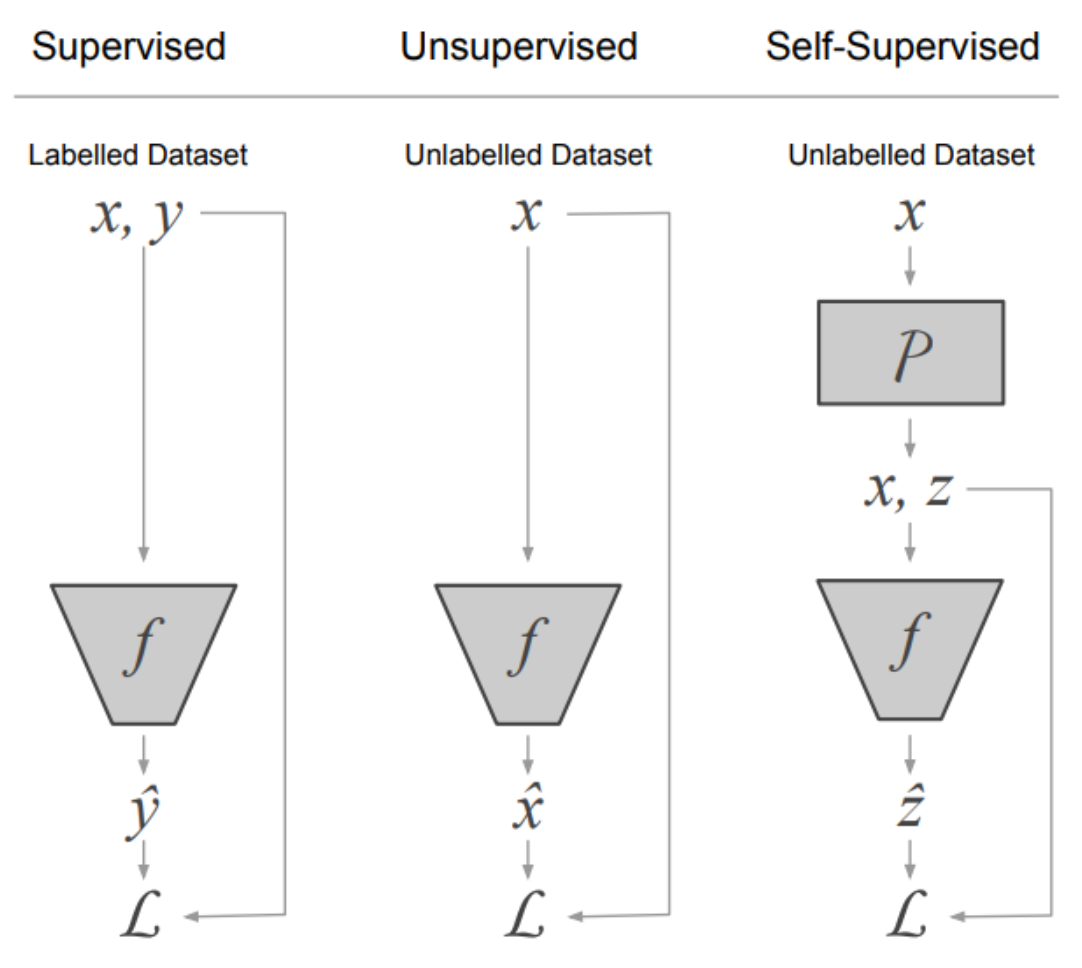
\includegraphics[width=0.5\textwidth]{img/lecture26/S US SSL.png}
    \caption{Comparison of supervised, unsupervised, and self-supervised learning pipelines and their sources of supervision.}
    \label{fig:ssl-comparison}
\end{figure}

As illustrated in Fig.~\ref{fig:ssl-comparison}, the primary difference between modern learning paradigms lies in how supervisory signals are obtained and how models are trained.

\subsection*{Supervised Learning}

\textbf{Supervised learning} relies on explicitly labeled datasets consisting of input–output pairs $(x,y)$, where $x$ represents the input data and $y$ denotes the corresponding ground-truth label. The primary objective is to learn a mapping function $f(x)\rightarrow y$ that generalizes well to unseen data. During training, the model parameters are optimized by minimizing a task-specific \textbf{loss function} $L(\hat{y},y)$ that measures the discrepancy between predictions and true labels. While this paradigm often achieves strong performance, it requires large quantities of high-quality labeled data, which can be expensive and time-consuming to obtain.

\subsection*{Unsupervised Learning}

\textbf{Unsupervised learning} operates without ground-truth labels and instead uses only unlabeled data $x$. The goal is to discover the underlying \textbf{structure}, \textbf{patterns}, or \textbf{distribution} of the data. A common formulation involves learning a mapping $f(x)\rightarrow\hat{x}$ that reconstructs the input, as in autoencoders. The model is trained by minimizing a reconstruction-based or distributional loss $L(\hat{x},x)$, encouraging the learned representation to capture meaningful properties of the data. This paradigm eliminates the need for labeled datasets, but it does not explicitly define the downstream task during training.

\subsection*{Self-Supervised Learning}

\textbf{Self-supervised learning (SSL)} bridges the gap between supervised and unsupervised learning by creating supervisory signals directly from unlabeled data. Instead of relying on manual annotations, SSL introduces carefully designed \textbf{pre-text tasks} that automatically generate \textbf{pseudo-labels} $z$ from the raw data $x$. The model first learns useful representations by solving these auxiliary tasks and is later \textbf{fine-tuned} on a downstream task using a smaller labeled dataset. The key distinction between SSL and unsupervised learning is the presence of structured supervisory signals derived from the data itself, enabling the model to learn more task-relevant and transferable representations \cite{1}.

\section{Self-Supervised Learning (SSL) Structure}

Self-supervised learning (SSL) follows a three-stage pipeline designed to learn powerful representations from large-scale unlabeled data and then adapt them to downstream tasks. The process consists of pseudo-label generation, self-supervised pre-training, and supervised fine-tuning.

\subsection*{Generate Pseudo-Labels}

\begin{figure}[H]
    \centering
    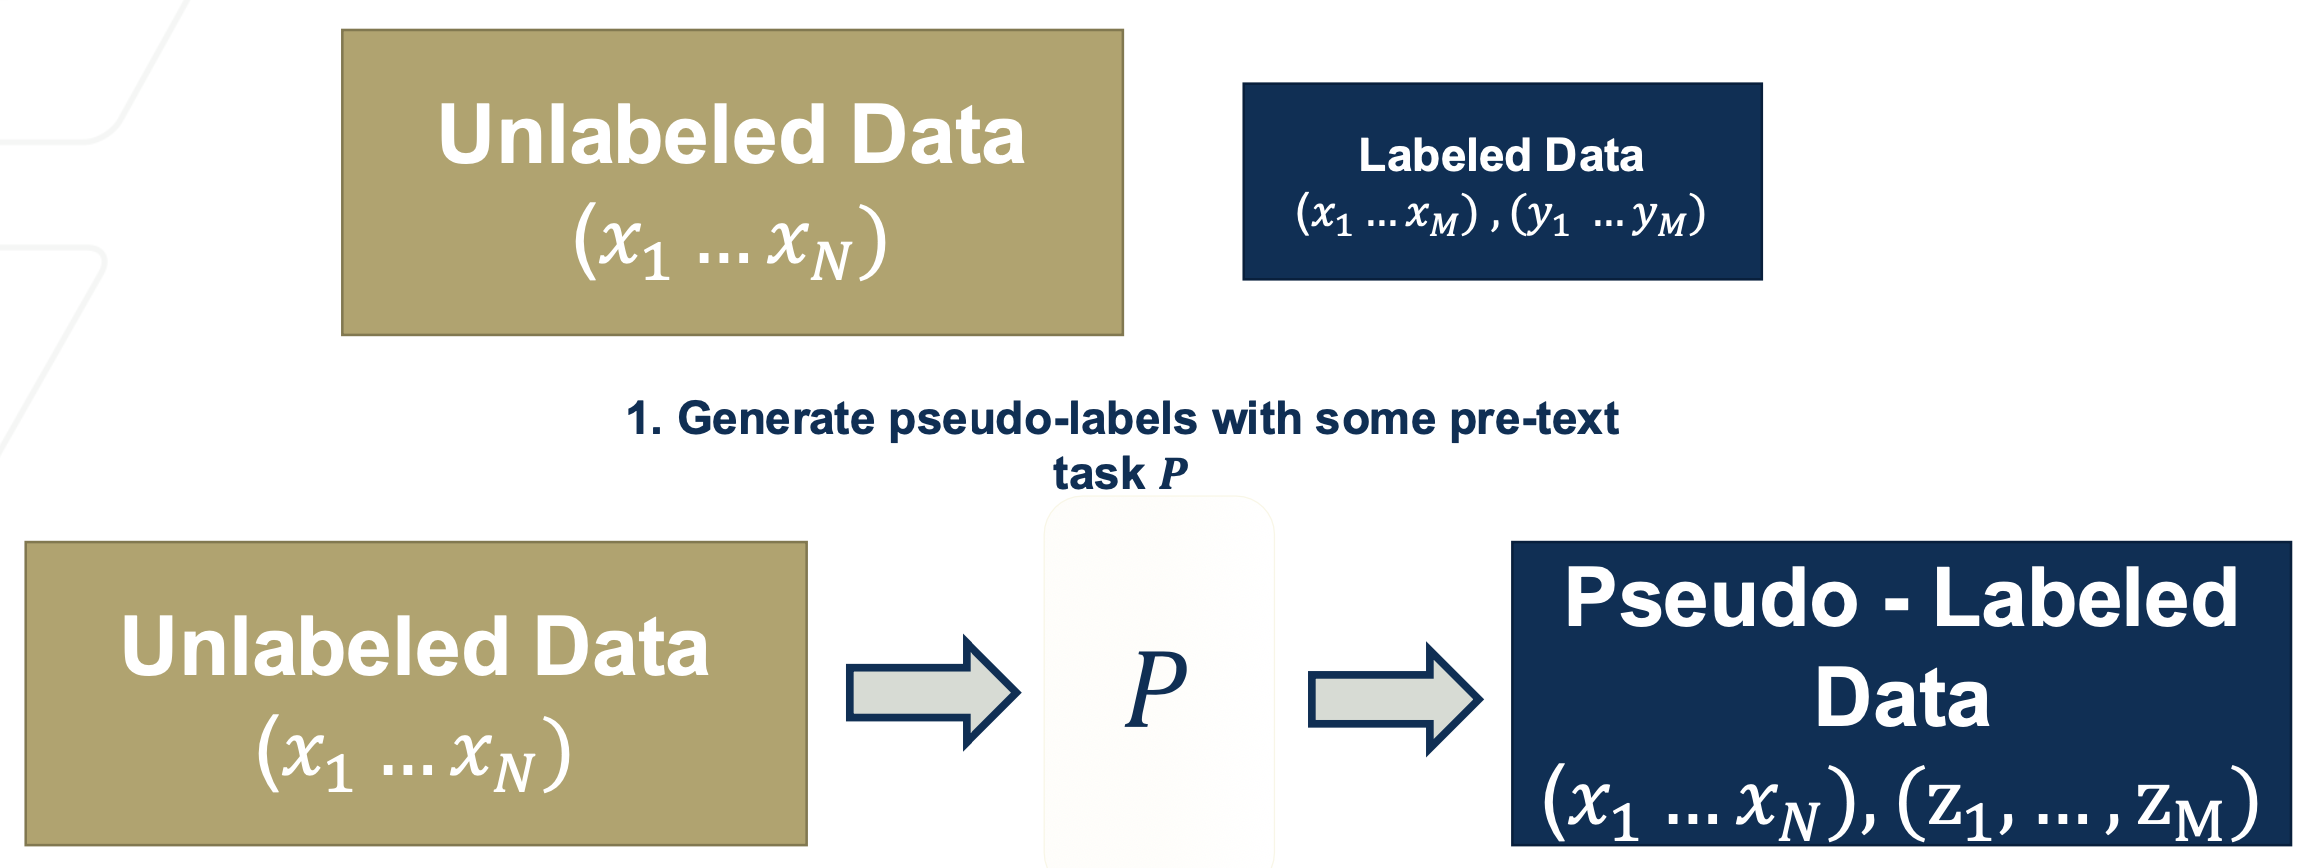
\includegraphics[width=0.7\textwidth]{img/lecture26/gen pseudo lab.png}
    \caption{Pseudo-label generation using a pre-text task.}
    \label{fig:pseudo-label-generation}
\end{figure}

The first stage focuses on constructing artificial supervision directly from \textbf{unlabeled data}. Given a large dataset $(x_1,\dots,x_N)$, a carefully designed \textbf{pre-text task} $P$ is applied to automatically generate \textbf{pseudo-labels} $(z_1,\dots,z_N)$. These pseudo-labels act as training targets without requiring human annotation. In some scenarios, a small labeled dataset $(x_1,\dots,x_M),(y_1,\dots,y_M)$ may also be available, but it is not required at this stage. The output of this step is a new pseudo-labeled dataset $(x_1,\dots,x_N),(z_1,\dots,z_N)$ that enables supervised-style training. Fig.~\ref{fig:pseudo-label-generation} illustrates how pre-text tasks transform unlabeled data into pseudo-labeled data.

\subsection*{Pre-Training on Pseudo-Labels}

\begin{figure}[H]
    \centering
    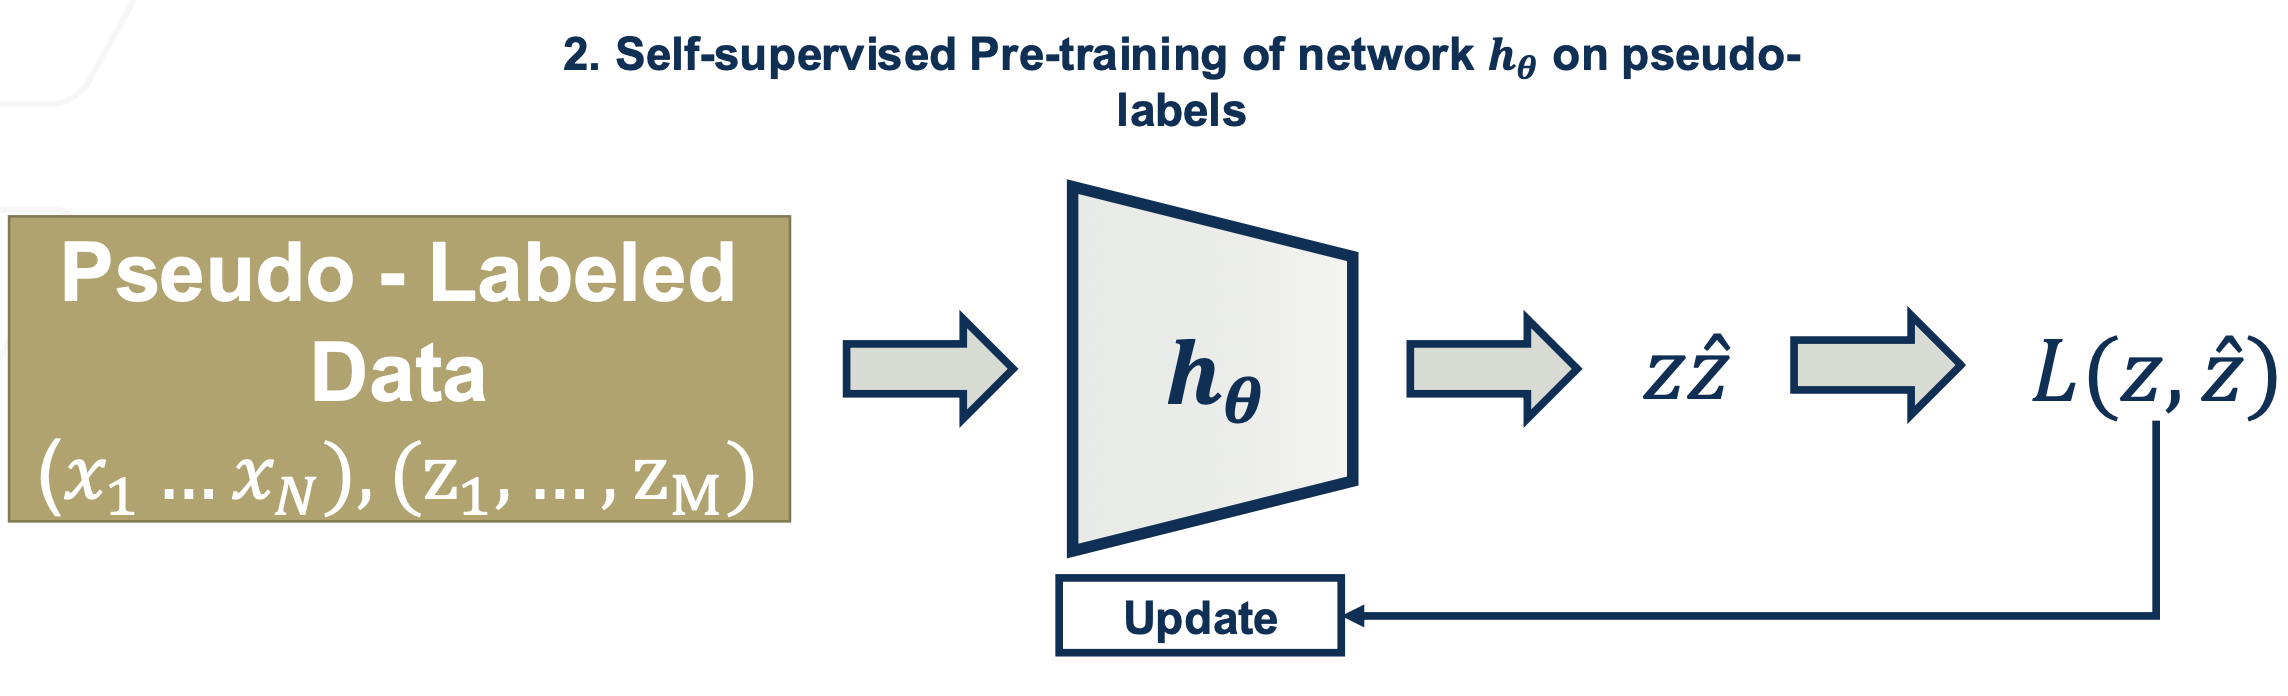
\includegraphics[width=0.7\textwidth]{img/lecture26/pre train on pse.png}
    \caption{Self-supervised pre-training using pseudo-labels.}
    \label{fig:ssl-pretraining}
\end{figure}

In the second stage, the pseudo-labeled dataset is used to train a neural network $h_\theta$. The network learns to predict pseudo-labels by minimizing a \textbf{self-supervised loss} $L(z,\hat{z})$, where $z$ represents the pseudo-label and $\hat{z}$ is the predicted output. This step is known as \textbf{self-supervised pre-training}. The goal is not to solve the final task directly, but rather to learn a general and transferable \textbf{representation} that captures meaningful structure in the data. After this stage, the network $h_\theta$ becomes a powerful feature extractor trained using large-scale unlabeled data, as shown in Fig.~\ref{fig:ssl-pretraining}.

\subsection*{Fine-Tuning for Downstream Tasks}

\begin{figure}[H]
    \centering
    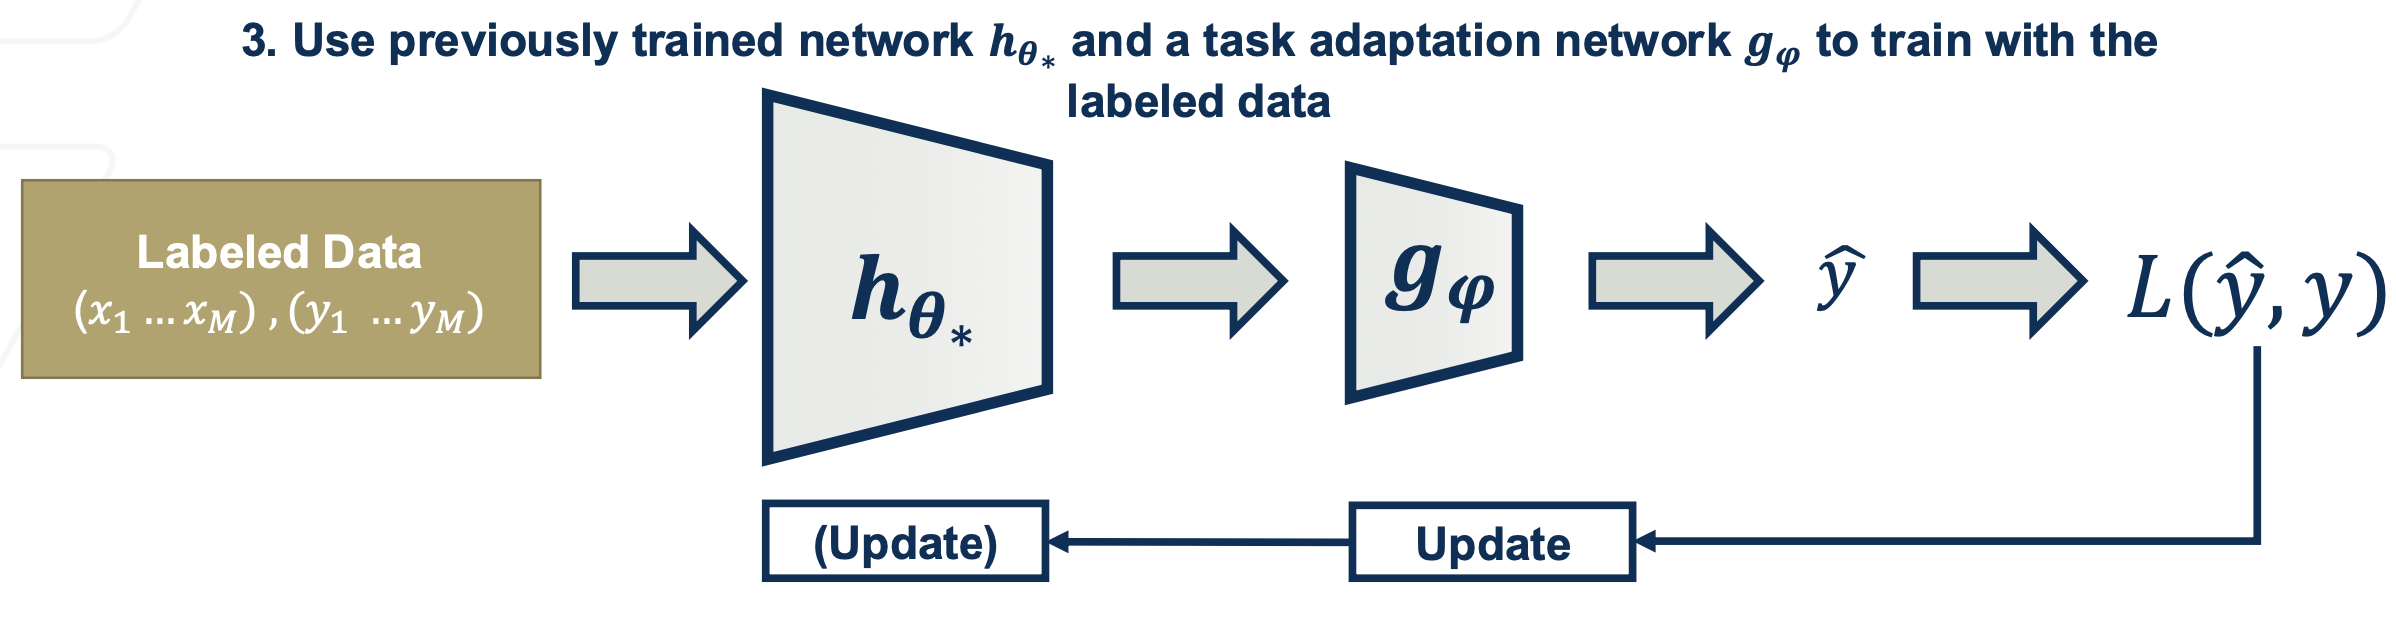
\includegraphics[width=0.7\textwidth]{img/lecture26/utilize learn model.png}
    \caption{Fine-tuning the pre-trained model for downstream tasks.}
    \label{fig:ssl-finetuning}
\end{figure}

The final stage adapts the learned representation to a specific \textbf{downstream task}. The pre-trained network $h_{\theta^*}$ is reused either as a fixed \textbf{feature extractor} or as an initialization for further training. A task-specific head $g_\phi$ (for example, a classifier) is attached and trained using labeled data $(x_1,\dots,x_M),(y_1,\dots,y_M)$. The model is optimized using a standard supervised loss $L(\hat{y},y)$. This step is called \textbf{fine-tuning} and enables strong performance even when labeled data is limited. Fig.~\ref{fig:ssl-finetuning} shows how the pre-trained network is adapted to downstream tasks.

\section{Different Pre-text Tasks in Self-Supervised Learning}

Self-supervised learning relies on carefully designed \textbf{pre-text tasks} to create supervisory signals directly from unlabeled data. These tasks encourage models to learn meaningful visual representations before being adapted to downstream tasks. Unlike traditional unsupervised learning, which often relies on generic reconstruction or density estimation, pre-text tasks provide \textbf{targeted supervision} that guides representation learning toward useful semantic features.

\subsection{Transformation Prediction}

\begin{figure}[H]
    \centering
    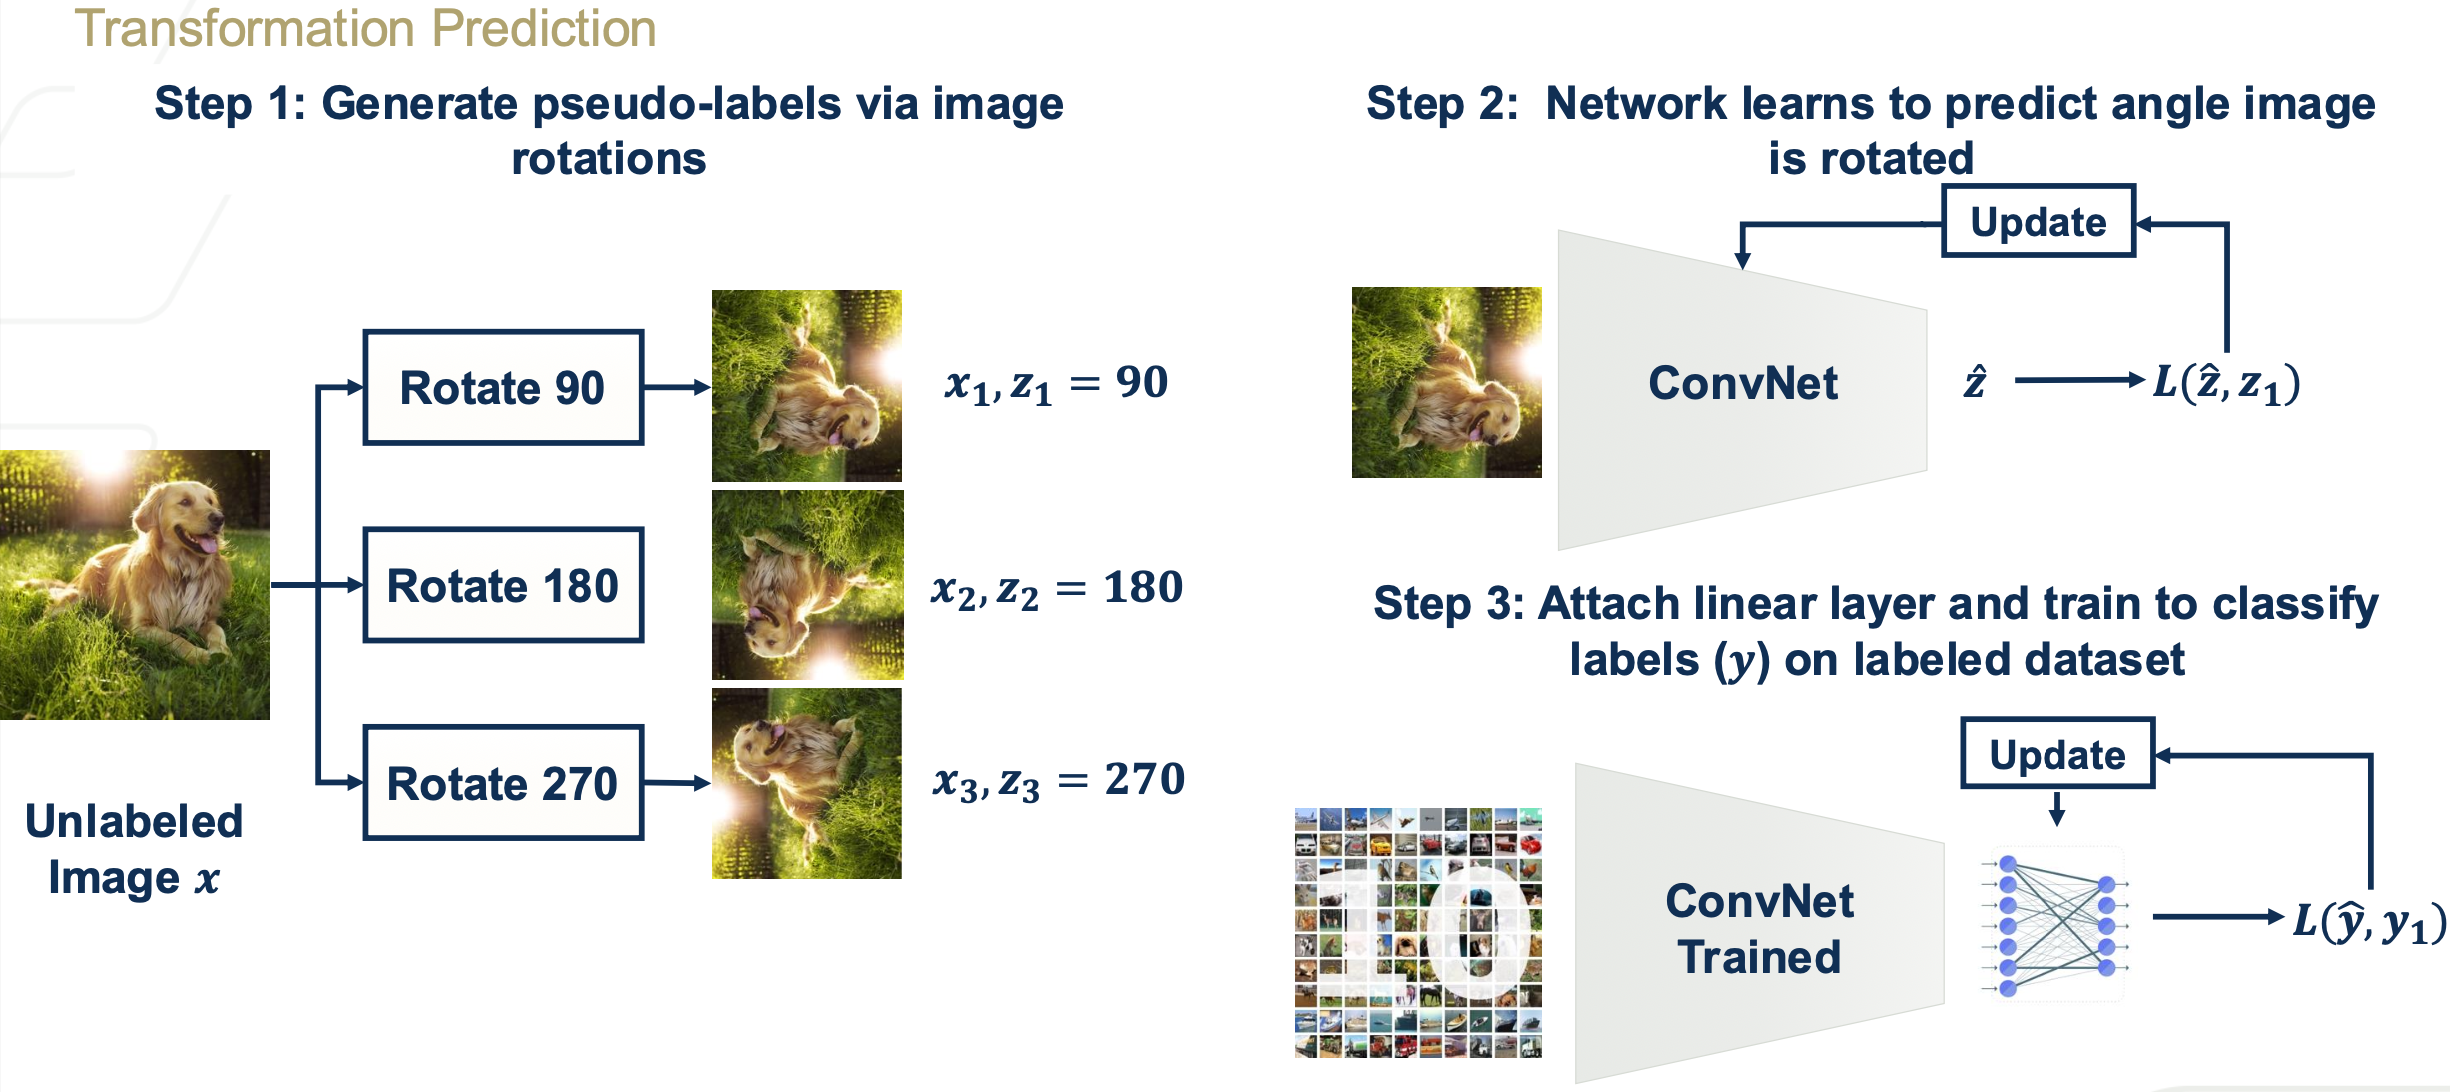
\includegraphics[width=0.7\textwidth]{img/lecture26/tran.png}
    \caption{Transformation prediction using image rotations as pseudo-labels.}
    \label{fig:ssl-rotation}
\end{figure}

\textbf{Transformation prediction} applies known transformations to input data and trains the model to identify which transformation was applied. The transformation itself becomes the \textbf{pseudo-label}. For example, an image can be rotated by $90^\circ$, $180^\circ$, or $270^\circ$, and the model is trained to predict the rotation angle. To perform well, the network must understand the \textbf{semantic structure} of the image (e.g., object orientation and shape). As illustrated in Fig.~\ref{fig:ssl-rotation}, the learned representation can later be reused for downstream classification tasks.

\subsection{Masked Prediction}

\begin{figure}[H]
    \centering
    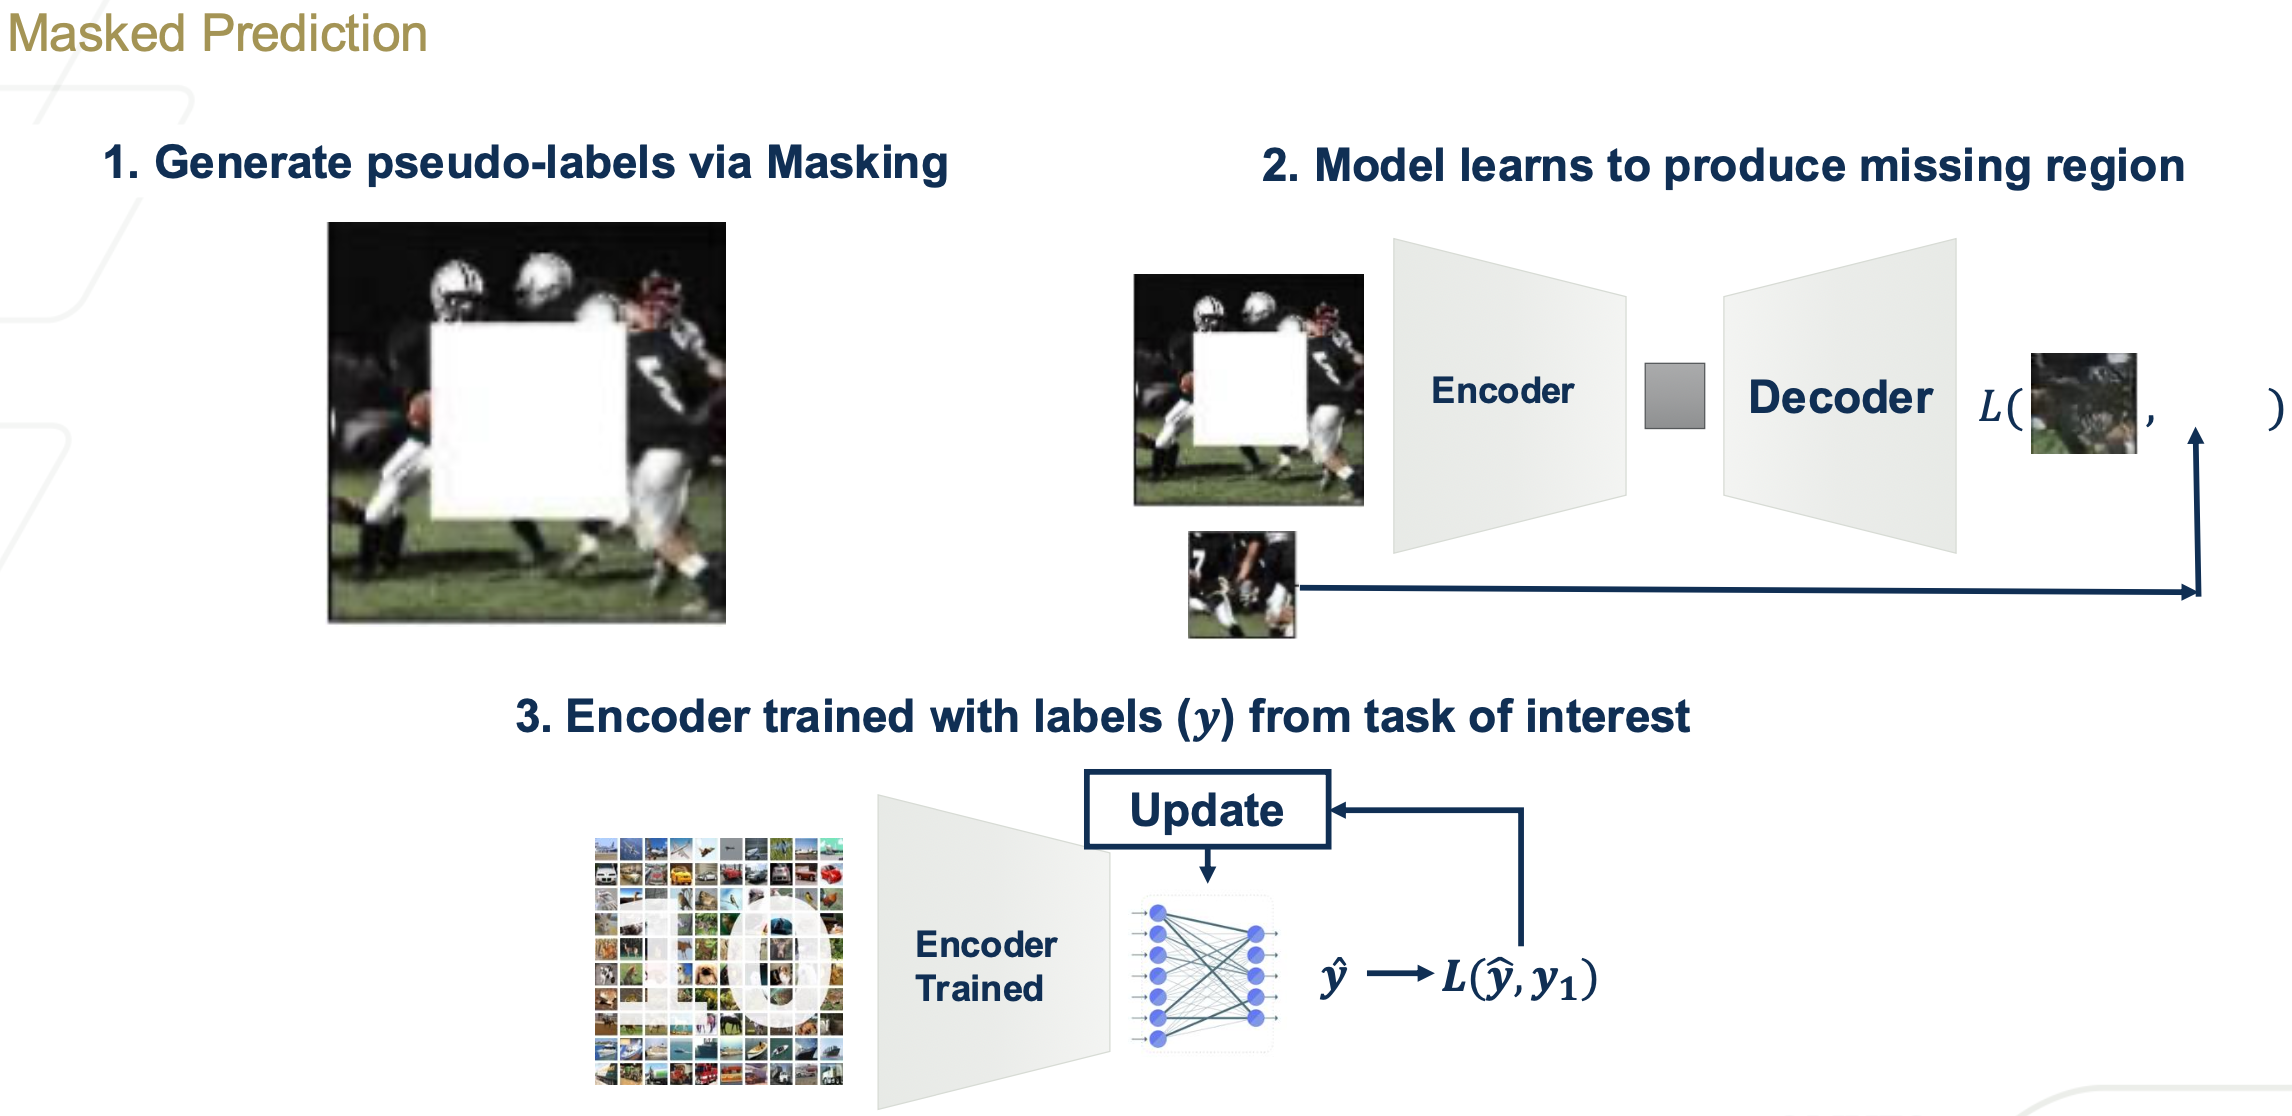
\includegraphics[width=0.7\textwidth]{img/lecture26/mask.png}
    \caption{Masked prediction using an encoder–decoder architecture.}
    \label{fig:ssl-masking}
\end{figure}

\textbf{Masked prediction} removes a portion of the input and trains the model to reconstruct the missing content. This forces the network to learn \textbf{contextual and structural relationships} within the data. A common approach masks a region of an image and trains an encoder–decoder architecture to predict the missing pixels. This idea is the foundation of many modern models, including masked autoencoders and language models such as BERT \cite{3, 6}. Fig.~\ref{fig:ssl-masking} illustrates how the network learns to reconstruct missing regions.

\subsection{Deep Clustering}

\begin{figure}[H]
    \centering
    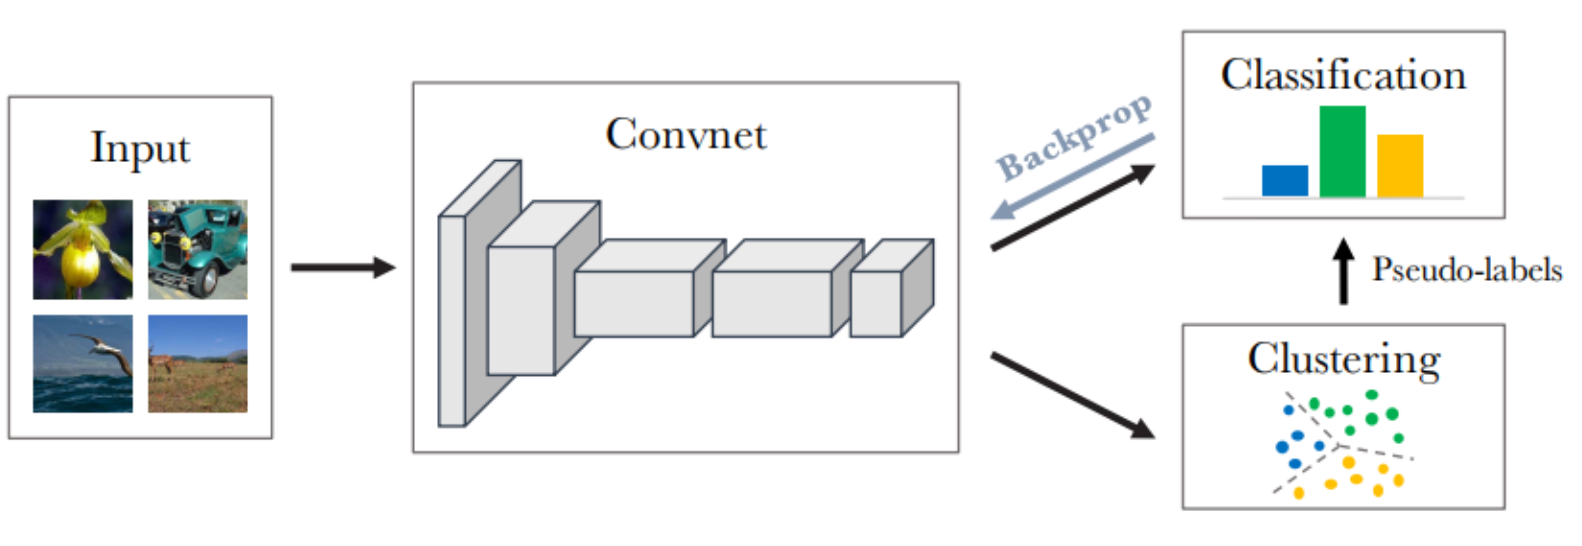
\includegraphics[width=0.7\textwidth]{img/lecture26/cluster.png}
    \caption{Deep clustering for generating pseudo-labels from feature clusters.}
    \label{fig:ssl-clustering}
\end{figure}

\textbf{Deep clustering} combines representation learning with clustering algorithms to iteratively generate pseudo-labels. First, features are extracted from unlabeled data using a neural network. These features are then grouped into clusters, and the cluster assignments are treated as pseudo-labels for supervised training. The network is retrained using these pseudo-labels, and the process is repeated. Over time, this iterative procedure refines the representation and improves clustering quality. The overall workflow is illustrated in Fig.~\ref{fig:ssl-clustering}.

\subsection{Contrastive Learning}

\begin{figure}[H]
    \centering
    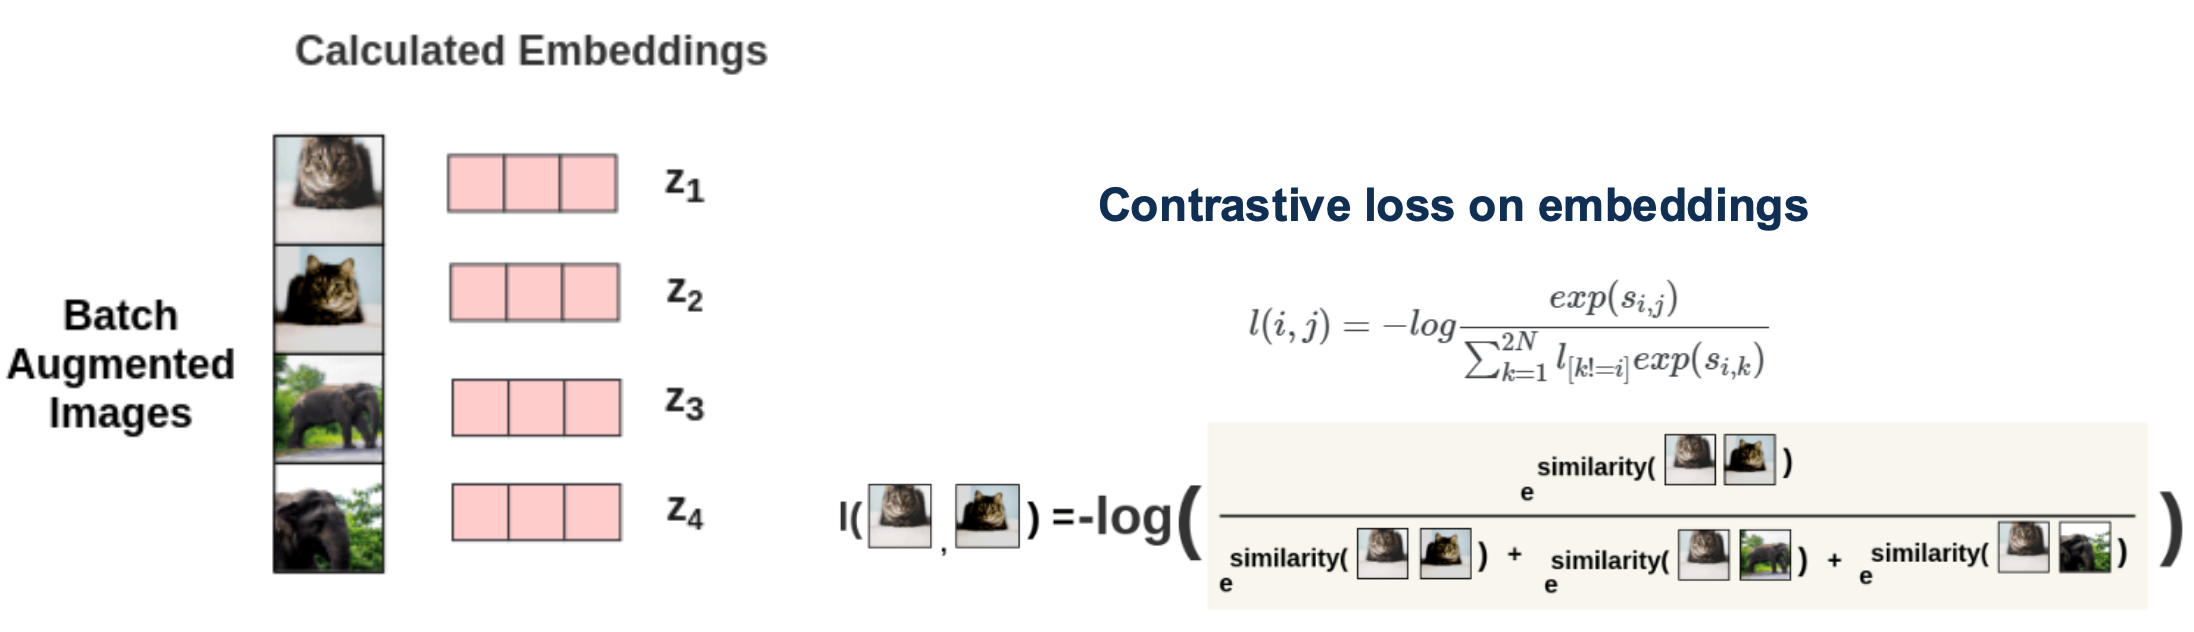
\includegraphics[width=0.7\textwidth]{img/lecture26/cont.png}
    \caption{Contrastive learning using positive and negative pairs of data.}
    \label{fig:ssl-contrastive}
\end{figure}

\textbf{Contrastive learning} has become one of the most influential self-supervised approaches \cite{2}. The core idea is to learn representations by comparing \textbf{positive pairs} and \textbf{negative pairs}. Positive pairs are different augmentations of the same data point, while negative pairs are augmentations from different data points. The model is trained using a \textbf{contrastive loss} that maximizes similarity between positive pairs and minimizes similarity between negative pairs. As shown in Fig.~\ref{fig:ssl-contrastive}, this encourages the model to learn invariant and highly discriminative feature representations. This topic will be explored in more detail in the following section.

\section{Self-Supervised Learning Objectives and Loss Functions}

\subsection{Contrastive Objectives and InfoNCE Loss}

A central idea in modern self-supervised learning is the use of contrastive objectives, which aim to learn representations by distinguishing between positive and negative pairs of data. One of the most widely used formulations is the InfoNCE loss.

Given an anchor sample $x_i$, a positive sample $x_j$ (an augmented view of the same data point), and a set of negative samples $\{x_k\}$ from different data points, the InfoNCE loss is defined as:

\begin{equation}
\mathcal{L}_{\text{InfoNCE}} = -\log \frac{\exp(\text{sim}(z_i, z_j)/\tau)}{\sum_{k} \exp(\text{sim}(z_i, z_k)/\tau)}
\end{equation}

where $\text{sim}(\cdot,\cdot)$ denotes cosine similarity and $\tau$ is a temperature parameter.

This objective encourages representations of positive pairs to be close while pushing apart representations of negative pairs. InfoNCE forms the foundation of many contrastive learning methods, including SimCLR, MoCo v2, and NNCLR, which differ primarily in how positive and negative pairs are constructed and sampled.

The effectiveness of InfoNCE has led to a family of contrastive self-supervised methods that rely on explicit negative samples. However, reliance on negative samples introduces challenges such as sampling bias and large batch requirements. This motivates alternative formulations that do not require negative pairs.

\subsection{Decorrelation-Based Objectives}

An alternative approach to self-supervised learning avoids the use of negative samples entirely. Instead, these methods enforce statistical constraints on learned representations, such as variance preservation and feature decorrelation.

A representative formulation includes objectives that:

\begin{itemize}
\item Encourage invariance between representations of augmented views
\item Maintain sufficient variance across feature dimensions
\item Reduce redundancy by decorrelating features
\end{itemize}

These principles lead to losses used in methods such as VICReg and Barlow Twins.

A representative decorrelation-based loss can be written as a combination of three terms:

\begin{equation}
\mathcal{L} = \mathcal{L}_{\text{inv}} + \mathcal{L}_{\text{var}} + \mathcal{L}_{\text{cov}}
\end{equation}

where:
\begin{itemize}
\item $\mathcal{L}_{\text{inv}}$ enforces similarity between augmented views,
\item $\mathcal{L}_{\text{var}}$ ensures each feature dimension has sufficient variance,
\item $\mathcal{L}_{\text{cov}}$ penalizes correlations between feature dimensions.
\end{itemize}

Together with contrastive objectives based on InfoNCE introduced earlier, these decorrelation-based objectives define two major families of self-supervised learning methods, which will be explored through representative frameworks in the following section.

\subsection{Relation to Anomaly and OOD Detection}

It is important to distinguish self-supervised learning (SSL) from related concepts such as anomaly detection and out-of-distribution (OOD) detection.

SSL focuses on learning meaningful representations from unlabeled data by solving pretext tasks (e.g., contrastive or reconstruction-based objectives). The goal is not to explicitly identify anomalies or detect distributional shifts, but rather to learn features that capture the underlying structure of the data. However, learning a structured representation does not guarantee separation between normal and anomalous samples, since SSL objectives are not explicitly designed to model rarity or distributional boundaries.

In contrast:
\begin{itemize}
    \item \textbf{Anomaly detection} aims to identify rare or unusual samples that deviate from normal patterns.
    \item \textbf{OOD detection} focuses on identifying inputs that fall outside the training distribution.
\end{itemize}

Although SSL does not directly solve these problems, the representations learned through SSL are often used as a foundation for downstream tasks such as anomaly detection and OOD detection, where better feature representations can significantly improve performance.

\section{Contrastive Learning Frameworks}

After introducing contrastive learning as an important \textbf{pre-text task}, we now examine a widely used practical framework and its impact on modern machine learning systems.

\subsection{SimCLR Framework}

\begin{figure}[H]
    \centering
    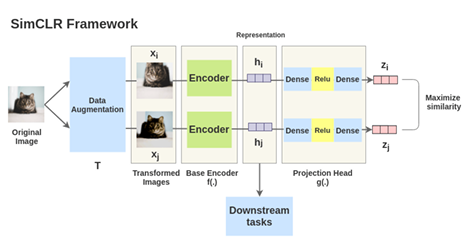
\includegraphics[width=0.7\textwidth]{img/lecture26/SimCLR_Framework.png}
    \caption{Overview of the SimCLR contrastive learning pipeline.}
    \label{fig:simclr_framework}
\end{figure}

\textbf{SimCLR} is a representative contrastive learning framework built upon the InfoNCE objective, described in the previous section, that learns visual representations by constructing \textbf{positive and negative pairs} within a training batch \cite{2}. As illustrated in Fig.~\ref{fig:simclr_framework}, the method consists of several key stages.

First, \textbf{image augmentation} is applied to each input image to generate two different transformed views of the same sample. These augmented views form a \textbf{positive pair}, while augmented views from different images form \textbf{negative pairs}. 

Next, both augmented images are passed through a shared \textbf{encoder network} to produce latent representations $h_i$ and $h_j$. These representations are then processed by a small \textbf{projection head}, which maps them into a lower-dimensional embedding space, producing embeddings $z_i$ and $z_j$. 

The framework then performs \textbf{similarity computation} using cosine similarity between embeddings. Training is driven by the \textbf{InfoNCE contrastive loss}, which encourages embeddings of positive pairs to be close while pushing embeddings of negative pairs apart \cite{2}. Finally, the loss is averaged across the batch, enabling efficient \textbf{batch-based optimization}. After training, the projection head is discarded and the encoder is used for downstream tasks. 

\subsection{VICReg Framework}

While contrastive methods such as SimCLR rely on the InfoNCE loss, decorrelation-based objectives provide an alternative approach to self-supervised learning. VICReg (Variance-Invariance-Covariance Regularization) is a representative method built on this principle.

VICReg is based on three components:

\begin{itemize}
\item \textbf{Invariance:} Encourages representations of augmented views to be similar
\item \textbf{Variance:} Prevents collapse by maintaining sufficient variance across features
\item \textbf{Covariance:} Reduces redundancy by decorrelating feature dimensions
\end{itemize}

The overall loss is defined as:

\begin{equation}
\mathcal{L}_{\text{VICReg}} = \lambda \mathcal{L}_{\text{inv}} + \mu \mathcal{L}_{\text{var}} + \nu \mathcal{L}_{\text{cov}}
\end{equation}

Unlike contrastive methods, VICReg does not require negative samples and avoids representation collapse through explicit regularization terms.

\subsection{Performance Comparison: Contrastive vs. Supervised Learning}

\begin{figure}[H]
    \centering
    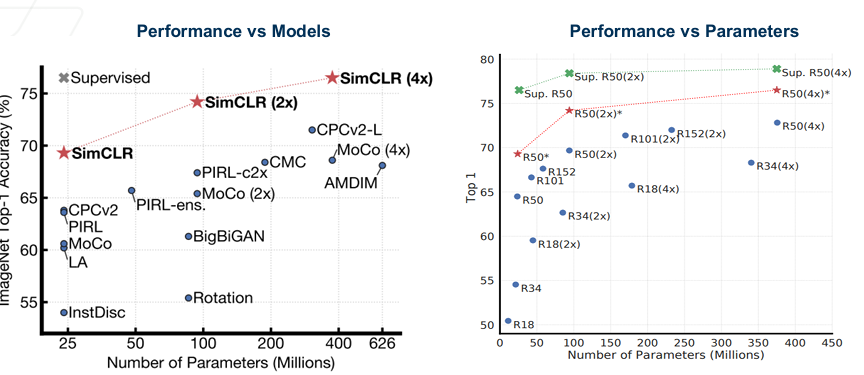
\includegraphics[width=0.7\textwidth]{img/lecture26/performance_comparison.png}
    \caption{Performance comparison between contrastive and supervised learning models.}
    \label{fig:contrastive_vs_supervised}
\end{figure}

Recent empirical results demonstrate that large-scale \textbf{contrastive learning} can rival or even surpass traditional \textbf{supervised learning} \cite{2}. As shown in Fig.~\ref{fig:contrastive_vs_supervised}, models trained using self-supervision achieve competitive ImageNet accuracy while using fewer labeled examples.

This shift has led to a \textbf{modern training paradigm} in which models are first trained using self-supervised objectives to learn general-purpose representations, and are then \textbf{fine-tuned} using supervised learning for specific tasks. Notably, many \textbf{foundation models} and \textbf{large language models} follow this training strategy, highlighting the growing importance of self-supervised learning at scale.

\section{Variations in Contrastive Learning Methods and Applications}

Contrastive learning is not defined by a single algorithm, but rather by a general principle: learning representations by distinguishing \textbf{positive pairs} from \textbf{negative pairs}. The primary variation across different methods lies in how these pairs are constructed. Depending on the data modality and task requirements, researchers design creative strategies to define meaningful supervisory signals. We now examine several representative applications that demonstrate the flexibility of contrastive learning.

\subsection{Core Concept}

The key differentiating factor among contrastive learning approaches is the strategy used to generate \textbf{positive and negative pairs}. In computer vision, positive pairs are often constructed using data augmentations of the same image. In domain-specific settings, however, positive relationships may be defined using spatial regions, temporal consistency, patient identity, or semantic similarity. Thus, contrastive learning adapts naturally to the structure of the data.

\subsection{Example Applications}

\subsubsection*{Fisheye Images}

\begin{figure}[H]
    \centering
    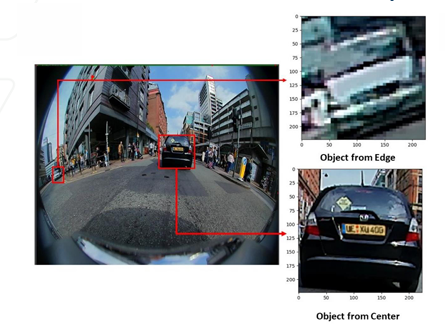
\includegraphics[width=0.7\textwidth]{img/lecture26/fisheye_region.png}
    \caption{Region-based contrastive learning in fisheye images.}
    \label{fig:fisheye_region}
\end{figure}

In fisheye image analysis, spatial distortion varies significantly across regions of the image. As shown in Fig.~\ref{fig:fisheye_region}, one approach treats different spatial regions as distinct semantic categories. 

Two complementary loss components can be defined:

\begin{itemize}
    \item $\mathbf{L_{\text{class}}}$: Objects of the same semantic class are treated as positive pairs, regardless of their spatial position.
    \item $\mathbf{L_{\text{region}}}$: Objects located in the same spatial region are treated as positive pairs, regardless of class.
\end{itemize}

These objectives are combined using a weighted loss:

\[
L = \alpha L_{\text{class}} + (1-\alpha) L_{\text{region}}
\]

Alternative partitioning strategies include square-based divisions, radial partitioning, or grid-wise segmentation, as illustrated in Fig.~\ref{fig:fisheye_alternative}.

\begin{figure}[H]
    \centering
    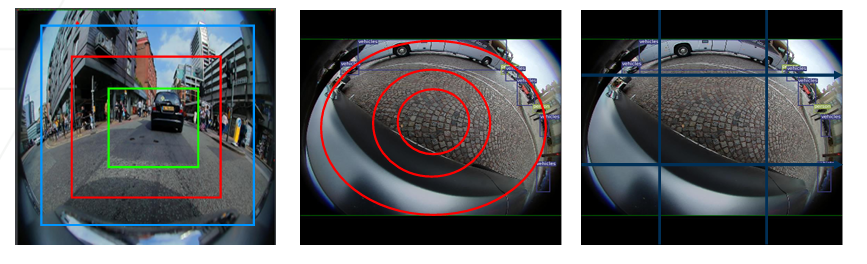
\includegraphics[width=0.7\textwidth]{img/lecture26/fisheye_alternative.png}
    \caption{Alternative region partitioning strategies for fisheye images.}
    \label{fig:fisheye_alternative}
\end{figure}

This example highlights how domain geometry influences pair construction.

\subsubsection*{Seismic Images}

\begin{figure}[H]
    \centering
    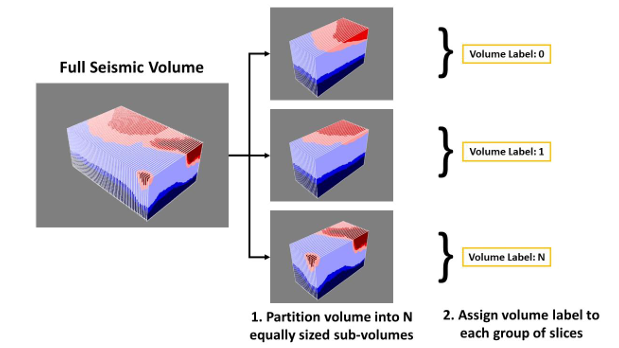
\includegraphics[width=0.7\textwidth]{img/lecture26/seismic.png}
    \caption{Contrastive learning via volume partitioning in seismic data.}
    \label{fig:seismic_contrastive}
\end{figure}

In seismic imaging, the data is volumetric rather than planar. As illustrated in Fig.~\ref{fig:seismic_contrastive}, the full seismic volume (e.g., $100 \text{ km} \times 100 \text{ km} \times 25 \text{ km}$) is partitioned into $N$ equal sub-volumes. Each sub-volume is assigned a pseudo-label, and slices from the same volume are treated as positive pairs.

This formulation transforms a structural geospatial property into a supervisory signal. The contrastive objective encourages the model to learn spatially consistent geological representations.

\subsubsection*{Medical Images}

\begin{figure}[H]
    \centering
    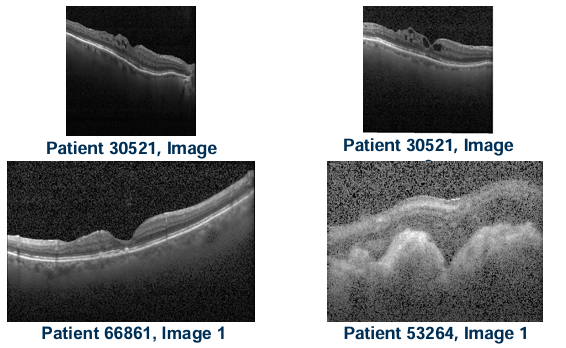
\includegraphics[width=0.7\textwidth]{img/lecture26/medical.png}
    \caption{Patient-based positive pair construction in medical imaging.}
    \label{fig:medical_contrastive}
\end{figure}

In medical imaging, positive and negative pairs can be defined using patient identity or clinical characteristics. As shown in Fig.~\ref{fig:medical_contrastive}, images from the same patient may be treated as positive pairs, while images from different patients form negative pairs. Alternatively, images sharing similar diagnoses can be grouped as positives.

This approach leverages domain-specific metadata to define meaningful similarity relationships.

\subsection{Contrastive Learning in Other Modalities}

\begin{figure}[H]
    \centering
    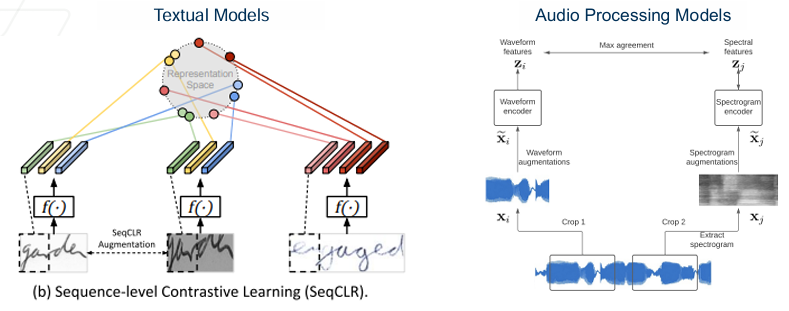
\includegraphics[width=0.7\textwidth]{img/lecture26/other_modalities.png}
    \caption{Contrastive learning applications in text and audio modalities.}
    \label{fig:contrastive_other_modalities}
\end{figure}

Although contrastive learning gained prominence in computer vision, it has been successfully extended to other modalities. In \textbf{textual models}, positive pairs may consist of different augmentations of the same sentence or semantically similar text spans. In \textbf{audio processing}, positive pairs can be constructed using different augmentations of the same waveform or spectrogram segment. Figure~\ref{fig:contrastive_other_modalities} illustrates representative architectures.

These examples demonstrate the \textbf{versatility and generality} of contrastive learning across diverse data types. The unifying principle remains the same: representations are learned by structuring similarity relationships within the data.

\section{Foundation Models}

Foundation models represent a major shift in modern machine learning \cite{4}. Instead of training task-specific models from scratch, large models are first trained on massive and diverse datasets using self-supervised objectives, and are later adapted to many downstream tasks. This paradigm connects directly to the self-supervised learning concepts discussed throughout this lecture.

\subsection{Recent Developments}

\begin{figure}[H]
    \centering
    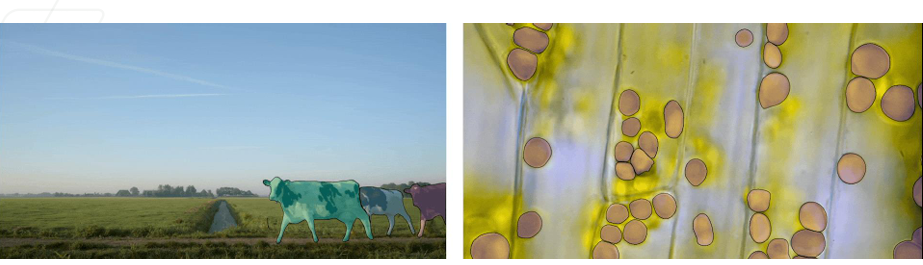
\includegraphics[width=0.7\textwidth]{img/lecture26/sam.png}
    \caption{Segment Anything Model (SAM): a large-scale foundation model for image segmentation.}
    \label{fig:sam}
\end{figure}

One prominent example of a modern foundation model is the \textbf{Segment Anything Model (SAM)}, released by Meta in April 2023 \cite{5}. As shown in Fig.~\ref{fig:sam}, SAM was trained on an unprecedented dataset containing \textbf{1.1 billion segmentation masks} from \textbf{11 million images}. This scale enables the model to generalize across diverse visual domains and perform segmentation without task-specific training.

\subsection{Historical Evolution}

The rise of foundation models can be understood through the evolution of deep learning architectures.

Prior to 2019, most computer vision systems relied on convolutional architectures such as \textbf{VGG} and \textbf{ResNet}. These models were typically trained in a fully supervised manner for specific tasks. 

After 2019, the field experienced a major transition with the introduction of \textbf{transformer-based architectures} and large-scale \textbf{self-supervised training}. Models such as \textbf{BERT}, \textbf{GPT}, \textbf{DALL-E}, and \textbf{Flamingo} demonstrated that training on massive unlabeled datasets could produce general-purpose representations adaptable to many tasks \cite{3,4}. This shift marks the emergence of the foundation model paradigm.

\subsection{Applications and Impact}

\begin{figure}[H]
    \centering
    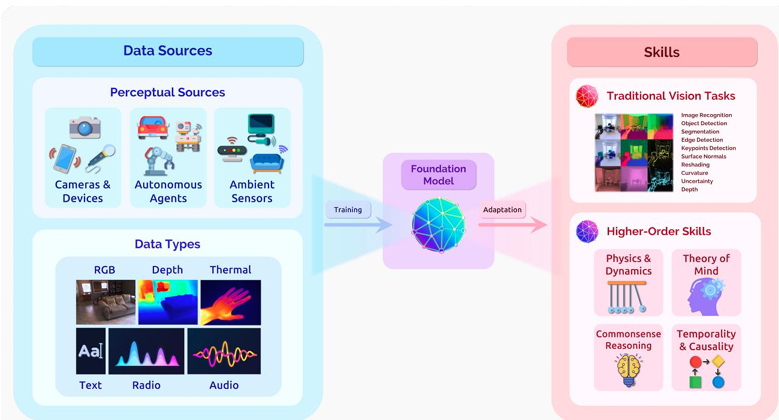
\includegraphics[width=0.7\textwidth]{img/lecture26/foundation_model.png}
    \caption{Foundation models trained on diverse multimodal data and adapted to downstream tasks.}
    \label{fig:foundation_models}
\end{figure}

Foundation models leverage \textbf{transfer learning at scale} \cite{4}. As illustrated in Fig.~\ref{fig:foundation_models}, these models are trained using diverse data sources and modalities, enabling the emergence of shared representations that transfer across tasks. Increasing model scale often leads to the emergence of higher-level reasoning and generalization capabilities.

The impact of foundation models spans many domains, including \textbf{healthcare}, \textbf{embodied interactive perception}, \textbf{visual knowledge distillation}, and \textbf{temporal and commonsense reasoning}. This paradigm represents the culmination of the ideas explored in this lecture: large-scale self-supervised learning enables the development of flexible, general-purpose AI systems.

\section{Key Insights and Conclusions}

\subsection{Pseudo-Label Generation}

A central idea of \textbf{self-supervised learning} is the design of effective \textbf{pseudo-labels}. The success of this paradigm relies heavily on the creativity used to construct meaningful pre-text tasks that generate supervisory signals directly from unlabeled data. Importantly, pseudo-labels must maintain a meaningful relationship with the true downstream labels so that the learned representations remain useful for real-world tasks. When designed properly, the features learned from pseudo-labels closely align with those required for supervised learning, enabling strong transfer and generalization.

\subsection{Future Directions}

Self-supervision at scale has become a fundamental component of modern AI systems. As datasets and model sizes continue to grow, \textbf{foundation models} trained using self-supervised objectives are expected to play an increasingly dominant role across domains. The continued evolution of these models will further expand their applications, shaping the future of machine learning and artificial intelligence.

\section{Q\&A Section}

\begin{enumerate}

\item \textbf{Question:} 
What is the main difference between \textbf{supervised}, \textbf{unsupervised}, and \textbf{self-supervised} learning in terms of where the supervision comes from?

\textbf{Solution:}  
In \textbf{supervised learning}, the supervision is provided by humans in the form of ground-truth labels $y$. The model learns a mapping from $x$ to $y$ by minimizing a loss between predictions and labels.  
In \textbf{unsupervised learning}, there are no labels at all — the model tries to discover structure directly from the data (for example, reconstruction or clustering).  
In \textbf{self-supervised learning}, the supervision is generated automatically from the data itself. A pre-text task creates \textbf{pseudo-labels} $z$ from the raw inputs $x$, and the model is trained to predict those pseudo-labels before being fine-tuned on a real task.

\item \textbf{Question:} 
Describe the three main stages of the self-supervised learning pipeline.

\textbf{Solution:}  
The pipeline has three steps.  
First, we \textbf{generate pseudo-labels} by applying a pre-text task to large amounts of unlabeled data. This turns raw data into a pseudo-labeled dataset.  
Second, we perform \textbf{self-supervised pre-training}, where a neural network learns to predict those pseudo-labels and becomes a strong feature extractor.  
Finally, we \textbf{fine-tune} the model on a downstream task using a smaller labeled dataset, adapting the learned representation to the final objective.

\item \textbf{Question:} 
How do \textbf{masked prediction} and \textbf{transformation prediction} differ in what they teach the model?

\textbf{Solution:}  
\textbf{Masked prediction} forces the model to fill in missing parts of the input, so it learns contextual relationships and global structure. The model has to understand how different parts of the data relate to each other.  
\textbf{Transformation prediction} asks the model to identify a known transformation (such as rotation). This encourages the model to learn semantic information like object orientation and shape.  
In short, masked prediction focuses on \emph{context}, while transformation prediction focuses on \emph{semantics and structure}.

\item \textbf{Question:} 
What are \textbf{positive pairs} and \textbf{negative pairs} in contrastive learning, and what is the goal of the contrastive objective?

\textbf{Solution:}  
Positive pairs are two different views of the \emph{same} sample (for example, two augmentations of the same image). Negative pairs come from \emph{different} samples.  
The goal is to learn representations where positive pairs are close together in the embedding space and negative pairs are far apart. This makes the representation both invariant to augmentations and discriminative across different inputs.

\item \textbf{Question:} 
Why does SimCLR use a \textbf{projection head} during training, and what part of the model is used later?

\textbf{Solution:}  
SimCLR first encodes images into representations and then maps them into a separate embedding space using a projection head. The contrastive loss works better in this projection space.  
After training, the projection head is removed, and the \textbf{encoder} is kept as the feature extractor for downstream tasks.

\item \textbf{Question:} 
What are \textbf{foundation models}, and why does \textbf{scale} matter so much for them?

\textbf{Solution:}  
Foundation models are large models trained on massive and diverse datasets so they can learn general-purpose representations. These models can then be adapted to many different tasks.  
Scale is critical because training on huge datasets with large models allows useful features and capabilities to \emph{emerge}. As a result, the model can transfer knowledge across tasks even with limited labeled data.

\item \textbf{Question:}
What is the goal of the InfoNCE loss in contrastive learning?

\textbf{Solution:}
The InfoNCE loss encourages the model to bring representations of positive pairs (different views of the same data point) closer together, while pushing representations of negative pairs (different data points) farther apart. This enables the model to learn invariant and discriminative feature representations.

\item \textbf{Question:}
How do decorrelation-based objectives such as VICReg avoid representation collapse without using negative samples?

\textbf{Solution:}
Decorrelation-based methods avoid collapse by enforcing three constraints: invariance, variance, and covariance. The invariance term aligns representations of augmented views, the variance term ensures that each feature dimension maintains sufficient spread, and the covariance term reduces redundancy between features. Together, these prevent trivial constant representations without requiring negative samples.

\end{enumerate}

\section{References}

\beginrefs

\bibentry{1}
Y. LeCun, Y. Bengio, and G. Hinton.
Deep learning.
Nature, 2015.

\bibentry{2}
T. Chen, S. Kornblith, M. Norouzi, and G. Hinton.
A Simple Framework for Contrastive Learning of Visual Representations.
ICML, 2020.

\bibentry{3}
J. Devlin, M. Chang, K. Lee, and K. Toutanova.
BERT: Pre-training of Deep Bidirectional Transformers.
NAACL, 2019.

\bibentry{4}
R. Bommasani et al.
On the Opportunities and Risks of Foundation Models.
arXiv, 2021.

\bibentry{5}
A. Kirillov et al.
Segment Anything.
ICCV, 2023.

\bibentry{6}
K. He et al.
Masked Autoencoders Are Scalable Vision Learners.
CVPR, 2022.

\endrefs

\end{document}